\documentclass[11pt,a4paper]{article}
\usepackage[utf8]{inputenc}
\usepackage[hmargin=2.0cm,vmargin=2.5cm,bindingoffset=0.5cm]{geometry}
\usepackage{amsfonts}
\usepackage{amsmath,amsthm,amssymb}
\allowdisplaybreaks
\usepackage{hyperref}
\usepackage{graphicx}
\usepackage{tikz}
\usepackage{mathtools}
\DeclarePairedDelimiter\ceil{\lceil}{\rceil}
\DeclarePairedDelimiter\floor{\lfloor}{\rfloor}
%\usepackage{float}
\usepackage{placeins}
\usepackage{diagbox}
\DeclareMathOperator{\Tr}{Tr}
\newtheorem{thm}{Theorem}
\usepackage{subcaption}
%\usepackage{subfigure}
\usepackage[english]{babel}
\author{Mohit}
\title{Quantum control of NV center using counter-diabatic driving  }
\begin{document}
\maketitle
%\tableofcontents

\section{Introduction}
The ground state of the NV center is a spin triplet with $| 0 \rangle, | -1 \rangle, | 1 \rangle$ spin sub-levels. They are defined in $S_z$ basis , where $\hat{z}$ direction is along the NV center axis. The Hamiltonian for the ground state of the NV center can be written as \cite{dhingra2017nitrogen}:
\begin{equation}
H_{NV}= \hbar \Delta S_z^2 + g \mu_B \vec{S}. \vec{B}_{ext} 
\end{equation}
where $\Delta= 2 \pi \times 2.87 $ GHz is zero-field splitting, $g \approx 2$ is the g-factor of electron in the NV center and $\mu_B$ is Bohr magneton. If there is no external magnetic field, then $| -1 \rangle$ and $| 1 \rangle$ levels are degenerate, and  $ \hbar^3 \Delta$ is the energy difference between $| 0 \rangle$ and $| \pm 1 \rangle$ energy levels.

\section{Eigenvalues}

Let's choose magnetic field to be in x-direction. Then we have:
\begin{align*}
H_{NV} &= \hbar \Delta S_z^2 + g \mu_B   S_x  B \\
 &= \Lambda S_z^2 + \lambda   S_x  
\end{align*}
where $\Lambda= \hbar \Delta $ and $\lambda=g \mu_B    B $. Magnetic field is going to be our control parameter in this problem. Using spin algebra  (appendix \ref{sec.spin_alegbra}), we obtain Hamiltonian in the $S_z$ basis ($|- 1\rangle$, $| 0 \rangle$ , $| 1 \rangle$):

\begin{equation}
H= \begin{bmatrix}
    \beta       & \alpha  & 0  \\
    \alpha       & 0 &\alpha  \\
     0       & \alpha & \beta
\end{bmatrix}
\end{equation}
where $\alpha= \hbar \lambda/ \sqrt{2} $ and $\beta= \hbar^2 \Lambda$.


\begin{figure}[!ht]
\begin{center}
\includegraphics[scale=0.5]{pics/energy_level_beta1.eps} 
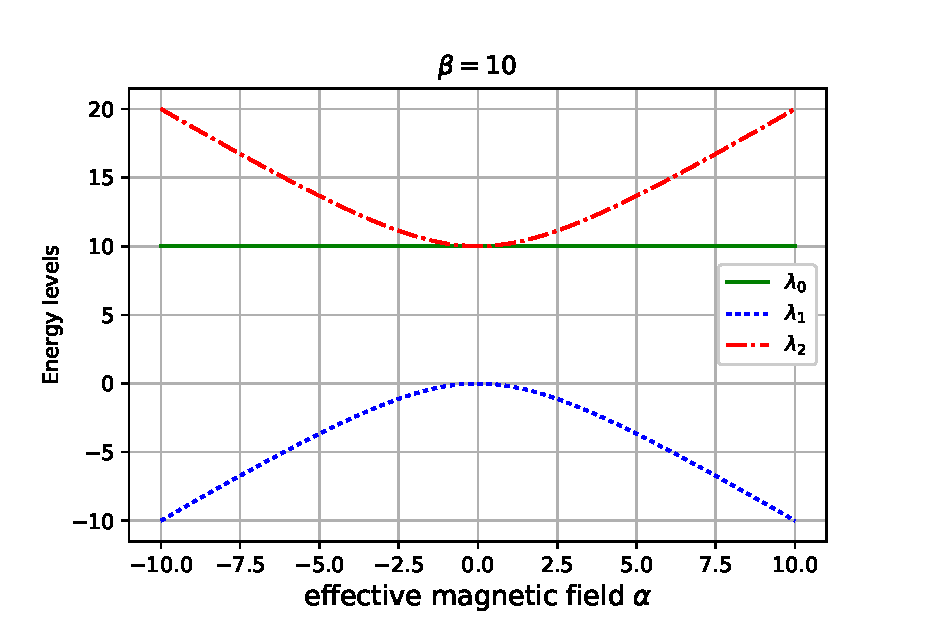
\includegraphics[scale=0.5]{pics/energy_level_beta10.eps} 
\caption{Avoided level crossing as a function of effective magnetic field }
\label{ev}
\end{center}
\end{figure}

 Energy eigenvalues are given by:
\begin{align*}
\lambda_0 &= \beta, \quad \lambda_1 = (\beta - \sqrt{\beta^2 + 8 \alpha^2})/2 , \quad  \lambda_2 = (\beta + \sqrt{\beta^2 + 8 \alpha^2})/2
\end{align*}
We should remember that $\alpha \propto B$. Hence, it makes sense that when $\alpha=0$,  there is a two -fold degeneracy and zero field energy gap is given by $\beta=\hbar^3 \Delta$. Now let's have a look at eigenvectors:
\begin{align*}
\nu_0 = (-1,0,1), \quad \nu_1 = (1, -(\beta + \sqrt{\beta^2 + 8 \alpha^2})/2 \alpha, 1) , \quad \nu_2 = (1, -(\beta - \sqrt{\beta^2 + 8 \alpha^2})/2 \alpha, 1)
\end{align*}

\section{Adiabatic gauge potential}

Now let's compute adiabatic gauge potential $A_{\lambda}= i \hbar \partial_{\lambda}$. Its' equation of motion is given by:
\begin{equation}
[H, \partial_{\lambda} H +\dfrac{i}{\hbar} [A_{\lambda}, H] ]=0
\end{equation}

We would choose a gauge such that diagonal elements of diabatic gauge potential $A_{\lambda}$ is zero. We can derive off- diagonal elements by using the identity $\langle m |H(\lambda) | n \rangle=0 \quad, n \neq m$ and then differentiate it with respect to $\lambda$ to obtain:
\begin{align}
\boxed{\langle m |A_{\lambda} | n \rangle =  -i \hbar \dfrac{\langle m |\partial_{\lambda}H | n \rangle}{E_m-E_n}}
\end{align}
where both  energies ($E_m, E_n$) and eigenvectors ($|m \rangle, |n \rangle$) depend on $\lambda$.

Here $\partial_{\lambda} H=S_x$ whose matrix representation is given in appendix \ref{sec.spin_alegbra}. After doing calculation in $S_z$ basis ($|- 1\rangle$, $| 0 \rangle$ , $| 1 \rangle$), we find that

\begin{equation}
A_{\lambda}=\hbar N
\begin{bmatrix}
0 & 0 & 0\\
0 & 0 & -i \\
0 & i & 0
\end{bmatrix}
\end{equation}
where N is given by
\begin{equation}
N=\dfrac{4\sqrt{2} \alpha \beta \hbar}{\sqrt{8 \alpha^{2} + \beta^{2}} \sqrt{8 \alpha^{2} + \left(\beta - \sqrt{8 \alpha^{2} + \beta^{2}}\right)^{2}} \sqrt{8 \alpha^{2} + \left(\beta + \sqrt{8 \alpha^{2} + \beta^{2}}\right)^{2}}}
\end{equation}

What I don't know is that the above gauge potential is composed of which spin operators. I am still working on it.

\subsection*{Expression involving commutators}

Another way to express this formula is:
\begin{equation}
 A_{\lambda}(\mu) =  -i\hbar \lim_{\mu \rightarrow 0} \sum_{n=0}^{\infty}   (-1)^{n} \dfrac{ C^{(2n+1)}}{\mu^{2n+2}}
\end{equation}
where $C^{(n)}$ is n- commutator of $H$ and $\partial_{\lambda} H$, i.e. $C^{(n)}= [H, [H, \mbox{ n times} \ldots,[H, \partial_{\lambda} H ]]] ] $.  We define the first term as $C^{(1)}= [H, \partial_{\lambda}H]$, second term as $C^{(2)}= [H,[H, \partial_{\lambda}H]]= [H, C^{(1)}]$ and so on and forth.

Let's find out $A_{\lambda}$ for this Hamiltonian for which we need to compute different odd-powered commutator $[H, \partial_{\lambda} H]$, where $\partial_{\lambda} H=S_x$. It turns out that I am not able to compute the summation as the expressions of commutators is pretty involved (details are given in appendix \ref{sec.potn}). I would need to think of some smarter way to compute adiabatic gauge potential.



\appendix

\section{Computation of gauge potential}\label{sec.potn}

Here we begin:
\begin{align*}
C^{(1)}=[H,S_x] &= \Lambda  [S_z^2, S_x] \\
&= S_z[S_z, S_x] + [S_z, S_x] S_z \\
&= i \hbar (S_z S_y + S_y S_z) \\
&=i \hbar ([S_z, S_y] +  2 S_y S_z)\\
&=i \hbar (- i \hbar S_x +  2 S_y S_z)
\end{align*}

\begin{align*}
C^{(2)}=[H,C^{(1)}] &=     \hbar^2 [H,  S_x]  +  i \hbar[ H,   S_y S_z] \\
&= \hbar^2 C^{(1)}  +  i \hbar S_y[ H,    S_z] +  i \hbar[ H,   S_y ]S_z\\
&= \hbar^2 C^{(1)}  +  i \hbar \lambda S_y [ S_x,    S_z] + i \hbar T\\
&= \hbar^2 C^{(1)} - \hbar^2 \lambda S_y^2  + i \hbar T
\end{align*}

\begin{align*}
T=[ H,   S_y ]S_z &= \Lambda [S_z^2, S_y]S_z + \lambda   [S_x, S_y]S_z   \\
 &=   \Lambda S_z[S_z, S_y]S_z+\Lambda [S_z, S_y]S_z^2 + i \hbar \lambda   S_z^2   \\
  &=  -i \hbar \Lambda  ( S_z S_x S_z+ S_x S_z^2) +  i \hbar \lambda   S_z^2   \\
    &=  -i \hbar \Lambda  ( [S_z, S_x] S_z+ 2 S_x S_z^2) +  i \hbar \lambda   S_z^2   \\
        &=  -i  \hbar \Lambda  ( i \hbar S_y S_z+ 2 S_x S_z^2) +  i \hbar \lambda   S_z^2   
\end{align*}
Hence, we get:
\begin{align*}
C^{(2)}=[H,C^{(1)}]  &= \hbar^2 C^{(1)}  -  \hbar^2 \lambda (S_y^2 +S_z^2)  + \hbar^2 \Lambda  ( i \hbar S_y S_z+  S_x S_z^2) \\
&= \hbar^2 C^{(1)}  -  \hbar^2 \lambda (S^2 - S_x^2)  + \hbar^2 \Lambda  ( i \hbar S_y S_z+  S_x S_z^2)
\end{align*}
Further, 
\begin{align*}
C^{(3)}=[H,C^{(2)}] &= [H,\hbar^2 C^{(1)}  -  \hbar^2 \lambda (S^2 - S_x^2)  + \hbar^2 \Lambda  ( i \hbar S_y S_z+  S_x S_z^2)] \\
&= \hbar^2  C^{(2)}  -  \hbar^2 \lambda [H,(S^2 - S_x^2)]   + \hbar^2 \Lambda  [H,( i \hbar S_y S_z+  S_x S_z^2)] \\
&= \hbar^2  C^{(2)} +  \hbar^2 \lambda [H, S_x^2]   +  i  \hbar^3 \Lambda  [H, S_y S_z] + \hbar^2 \Lambda  [H, S_x S_z^2] \\
&= \hbar^2  C^{(2)} +  \hbar^2 \lambda^2 [S_z^2, S_x^2]   +  i  \hbar^3 \Lambda T_1 + \hbar^2 \Lambda T_2 \\
&= \hbar^2  C^{(2)} +  \hbar^2 \lambda  T_0   +  i  \hbar^3 \Lambda T_1 + \hbar^2 \Lambda T_2 
\end{align*}

\begin{align*}
T_0 =[S_z^2, S_x^2]  &=S_z[S_z, S_x^2] + [S_z, S_x^2]S_z \\
					&=S_z S_x[S_z, S_x] + S_z [S_z, S_x]S_x + S_x[S_z, S_x]S_z + [S_z, S_x]S_xS_z \\
					&=i \hbar(S_z S_xS_y + S_z S_yS_x + S_xS_yS_z + S_y S_xS_z ) \\
					&=i \hbar(S_z [ S_x, S_y] + 2 S_z S_yS_x + [S_x, S_y] S_z + 2S_y S_xS_z ) \\
					&=2i \hbar (i \hbar S_z^2  + S_z S_y S_x   + S_y S_xS_z ) \\
					&=-2 \hbar^2 S_z^2  + 2i \hbar ( S_z S_y S_x   + S_y S_xS_z ) 
\end{align*}

\begin{align*}
T_1 =[H, S_y S_z]  = - \hbar^2 \lambda S_y^2  + i \hbar T &= - \hbar^2 \lambda S_y^2  +  \hbar^2 \Lambda  ( i \hbar S_y S_z+ 2 S_x S_z^2) - \hbar^2 \lambda   S_z^2\\
&= - \hbar^2 \lambda (S_y^2 + S_z^2) +  \hbar^2 \Lambda  ( i \hbar S_y S_z+ 2 S_x S_z^2) 
\end{align*}

\begin{align*}
T_2 =[H, S_x S_z^2] & = [H, S_x ]S_z^2 + S_x [H,  S_z^2] \\
 &= C^{(1)}S_z^2 + \lambda S_x [S_x,  S_z^2]  \\
&= C^{(1)}S_z^2 + \lambda S_x [S_x,  S_z]S_z + \lambda S_x S_z [S_x,  S_z]  \\
&= C^{(1)}S_z^2 - i \hbar  \lambda (S_x S_y S_z +  S_x S_z S_y)  \\
&= C^{(1)}S_z^2 - i \hbar  \lambda (S_x [S_y, S_z] + 2 S_x S_z S_y)  \\
&= C^{(1)}S_z^2 - i \hbar  \lambda (i \hbar S_x^2 + 2 S_x S_z S_y)  \\
&= C^{(1)}S_z^2 + \hbar^2  \lambda  S_x^2  - 2 i \hbar  \lambda  S_x S_z S_y
\end{align*}

Finally, we get 
\begin{align*}
C^{(3)}&=\hbar^2  C^{(2)} +  \hbar^2 \lambda  T_0   +  i  \hbar^3 \Lambda T_1 + \hbar^2 \Lambda T_2 \\
&=\hbar^2  C^{(2)} +  2i \hbar^3 \lambda  (i \hbar S_z^2  + S_z S_y S_x   + S_y S_xS_z )    +  \hbar^2 \Lambda( i  \hbar T_1 +  T_2) 
\end{align*}

 Let's simplify the last term $i  \hbar T_1 +  T_2$:
 \begin{align*}
 i  \hbar T_1 +  T_2 &= - i \hbar^3 \lambda (S_y^2 + S_z^2) +  i \hbar^3 \Lambda  ( i \hbar S_y S_z+ 2 S_x S_z^2) +  C^{(1)}S_z^2 + \hbar^2  \lambda  S_x^2  - 2 i \hbar  \lambda  S_x S_z S_y \\
 &= - i \hbar^3 \lambda (S_y^2 + S_z^2)   + \hbar^2  \lambda  S_x^2 + i \hbar^3 \Lambda  ( i \hbar S_y S_z+ 2 S_x S_z^2) - 2 i \hbar  \lambda  S_x S_z S_y +  C^{(1)}S_z^2 \\
 &= - i \hbar^3 \lambda (S_y^2 + S_z^2)   + \hbar^2  \lambda  S_x^2 + i \hbar^3 \Lambda  ( i \hbar S_y S_z+ 2 S_x S_z^2) - 2 i \hbar  \lambda  S_x S_z S_y +  i \hbar (- i \hbar S_x +  2 S_y S_z) S_z^2 \\
  &= - i \hbar^3 \lambda (S_y^2 + S_z^2)   + \hbar^2  \lambda  S_x^2 + i \hbar^3 \Lambda  ( i \hbar S_y S_z+ 2 S_x S_z^2) - 2 i \hbar  \lambda  S_x S_z S_y +  \hbar^2 S_x S_z^2 +  2  i \hbar S_y  S_z^3 \\
   &= - i \hbar^3 \lambda (S_y^2 + S_z^2)   + \hbar^2  \lambda  S_x^2 +  \hbar^2 S_x S_z^2 (1+ 2 i \hbar \Lambda)  - \hbar^4 \Lambda  S_y S_z - 2 i \hbar  \lambda  S_x S_z S_y   +  2  i \hbar S_y  S_z^3 \\
 \end{align*}
 Now, let's write:
 \begin{align*}
   C^{(2)}= \hbar^2 C^{(1)}  -  \hbar^2 \lambda (S^2 - S_x^2)  + \hbar^2 \Lambda  ( i \hbar S_y S_z+  S_x S_z^2)
 \end{align*}

\section{Spin Algebra}\label{sec.spin_alegbra}
\begin{equation}
[S_x, S_y]=i \hbar S_z, \quad [S_y, S_z]=i \hbar S_x \quad [S_z, S_x]=i \hbar S_y
\end{equation}
\begin{equation}
S^2|s ,m \rangle = \hbar^2 s(s+1)|s ,m\pm 1\rangle  \quad S_z|s ,m \rangle = \hbar m |s ,m \rangle
\end{equation}
\begin{equation}
S_{\pm}|s, m\rangle = \hbar\sqrt{s(s+1)-m(m \pm 1)}|s,m \pm 1\rangle
\end{equation}
where $S_+ = S_x + iS_y$ and $S_- = S_x - iS_y $. Hence, we get $S_x = (S_+ + S_-)/2$ and $S_y = (S_+ - S_-)/2i $

\begin{equation}
S_+= \sqrt{2} \hbar\begin{bmatrix}
0 & 1 & 0\\
0 & 0 & 1\\
0 & 0 & 0\\
\end{bmatrix}
\quad
S_-=\sqrt{2} \hbar 
\begin{bmatrix}
0 & 0 & 0\\
1 & 0 & 0\\
0 & 1 & 0\\
\end{bmatrix}
\end{equation}

Hence,
\begin{equation}
S_x= \frac{\hbar}{\sqrt{2} }
\begin{bmatrix}
0 & 1 & 0\\
1 & 0 & 1\\
0 & 1 & 0\\
\end{bmatrix} \quad
S_y=  i \frac{\hbar}{\sqrt{2} }
\begin{bmatrix}
0 & -1 & 0\\
1 & 0 & -1\\
0 & 1 & 0\\
\end{bmatrix}
\end{equation}


\bibliography{ref} 

\bibliographystyle{unsrt}
%\bibliographystyle{plain}

\end{document}
